% Provenance (never printed): cycle 3 / 6e "La planete Terre" (water in the
% ground, groundwater, springs and wells; resource); see
% sources/book1/PROVENANCE.md. Book 1, grade 6, chapter 5.
% Vocabulary guard: "sediment" not before g7.4; the water cycle is recalled
% from the physics book (prose only).
\chapter{地下的水}\label{ch:g6:water-underground}

在炎热的夏日，田野干涸，溪流水位很低。
然而在\omterm{def:g1:landscapes-around-us:landform}{丘陵}脚下，冷而清澈的水仍如整个冬天那样不断从地下涌出，
注满了一个水池。已经数周没有下雨了。这些水从哪里来，
又是如何从\omterm{def:g3:stones-pebbles-sand:rock}{岩石}中流出的？

\begin{omfigure}
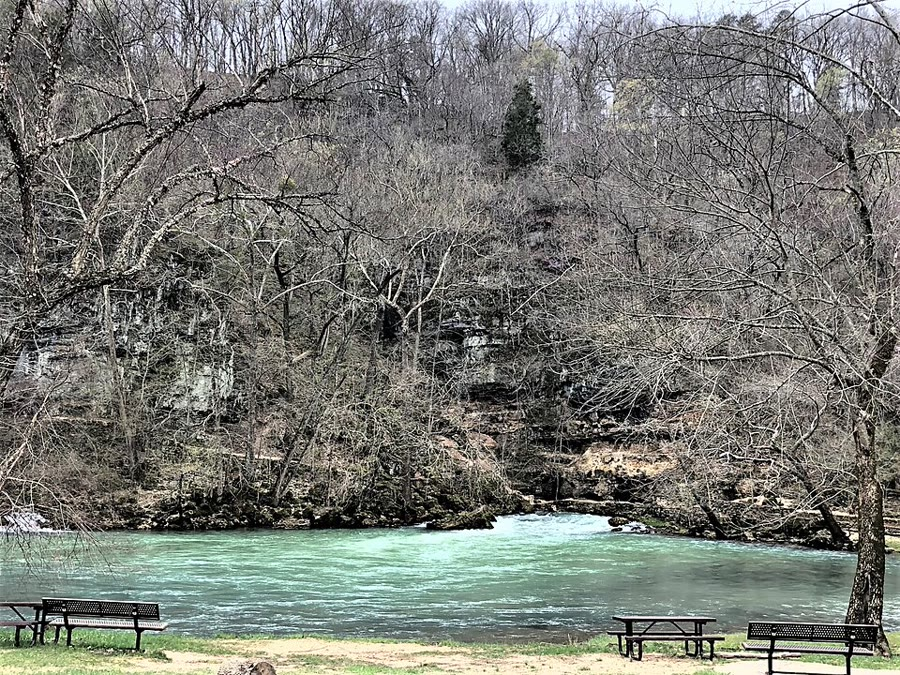
\includegraphics[width=0.72\linewidth]{images/book1/g6-big-spring.jpg}

{\small 泉水从岩壁脚下涌出并注满水池：大泉
（美国密苏里州）。（照片：Johnston9494, CC BY-SA 4.0，经
维基共享资源。）}
% ledger: commons:big-spring
\end{omfigure}

\begin{recall}
地球上几乎所有的水都是\omterm{def:g2:water-on-earth:salt-fresh}{咸水}，\omterm{def:g2:water-on-earth:salt-fresh}{淡水}只占很小一部分，
其中大部分以冰的形式存在，或埋藏于地下
（见\cref{ch:g2:water-on-earth}）。砂岩和石灰岩等\omterm{def:g3:stones-pebbles-sand:rock}{岩石}
由颗粒或贝壳胶结而成，黏土和页岩则由
极细的颗粒组成（见\cref{ch:g6:rocks-and-minerals}）。在物理各册中，
你已经追踪过水在水循环中的路径：水从
\omterm{def:g2:water-on-earth:ocean}{海洋}蒸发，凝结成云，又以雨或雪的形式落下。
\end{recall}

\section{雨水下渗}

雨落到陆地上时，水有三条去向。一部分
蒸发回到空气中；一部分沿地表流动，顺着坡面
汇入溪流和\omterm{def:g1:landscapes-around-us:water}{河流}，这就是\emph{地表径流}。其余部分
渗入地下。

\begin{definition}[下渗]\label{def:g6:water-underground:infiltration}
\emph{下渗}\index{下渗}是指雨水或融雪
渗入地面，穿过土壤，向下进入\omterm{def:g3:stones-pebbles-sand:rock}{岩石}中。
\end{definition}

渗入多少水取决于地面状况。在陡坡上、裸露
或坚硬的地面上、道路或停车场上，或土壤已经
饱和时，大部分水都会流走。在缓坡上，草地、
树林下或沙质土壤上，更多的水有时间渗入。

\begin{omfigure}
\begin{tikzpicture}[x=1cm, y=1cm]
  % rain
  \foreach \x in {0.3,0.9,...,10.5} \draw[blue!55, thick] (\x,3.9) -- (\x-0.15,3.45);
  % ground: field on the left (gentle), road and town on the right
  \fill[brown!30] (0,0) -- (0,2.2) -- (5.2,1.9) -- (5.6,1.85) -- (10.8,1.1) -- (10.8,0) -- cycle;
  \draw[green!50!black, line width=2.5pt] (0,2.2) -- (5.2,1.9);
  \fill[gray!70] (5.6,1.85) -- (10.8,1.1) -- (10.8,0.98) -- (5.6,1.73) -- cycle;
  \foreach \x in {0.4,1.0,...,4.6} \draw[green!45!black, thick] (\x,{2.2-0.058*\x}) -- ++(0.05,0.28) (\x,{2.2-0.058*\x}) -- ++(-0.06,0.24);
  % infiltration arrows in the field
  \foreach \x in {0.8,1.9,3.0,4.1} \draw[->, blue!70!black, very thick] (\x,{2.0-0.058*\x}) -- ++(0,-1.0);
  \node[font=\scriptsize, blue!70!black, align=center, fill=brown!30] at (2.45,0.45) {下渗：水渗入地下};
  % run-off on the road
  \draw[->, blue!70!black, very thick] (6.0,2.05) -- (10.3,1.45);
  \node[font=\scriptsize, blue!70!black, align=center] at (8.3,2.3) {地表径流：水流走};
  \node[font=\scriptsize, align=center] at (8.3,0.5) {道路：地面坚硬，\\ 很少有水渗入};
  \node[font=\scriptsize] at (2.45,2.75) {草地};
  % evaporation
  \draw[->, gray, thick, decorate, decoration={snake, amplitude=1.2pt, segment length=5pt}] (4.9,2.2) -- (4.9,3.3);
  \node[font=\scriptsize, gray!60!black, anchor=west] at (5.0,3.0) {蒸发};
\end{tikzpicture}

{\small 雨水的三条去向。在草地上，大部分水会渗入；
在道路上，大部分水会流走。}
\end{omfigure}

\section{多孔岩石与透水性}

用手持放大镜看一把干燥的\omterm{def:g3:stones-pebbles-sand:sand}{沙子}：颗粒之间
有许多微小的空隙。向沙上倒水，水便会充满这些空隙。
许多\omterm{def:g3:stones-pebbles-sand:rock}{岩石}也是这样：颗粒之间布满了小孔洞，
或布满细小的裂缝。

\begin{definition}[孔隙度]\label{def:g6:water-underground:porosity}
\omterm{def:g3:stones-pebbles-sand:rock}{岩石}的\emph{孔隙}\index{孔隙}是指颗粒之间
和裂缝中的空隙。具有孔隙的\omterm{def:g3:stones-pebbles-sand:rock}{岩石}称为\emph{多孔的}\index{多孔的}。其
\emph{孔隙度}\index{孔隙度}是其体积中由孔隙构成的比例，
通常以百分数表示。
\end{definition}

\begin{definition}[透水性]\label{def:g6:water-underground:permeability}
当水能够流经\omterm{def:g3:stones-pebbles-sand:rock}{岩石}时，该\omterm{def:g3:stones-pebbles-sand:rock}{岩石}是\emph{透水的}\index{透水的}，
因为其\omterm{def:g6:water-underground:porosity}{孔隙}足够大且彼此相连。
水无法流过时，\omterm{def:g3:stones-pebbles-sand:rock}{岩石}是\emph{不透水的}\index{不透水的}。
\emph{透水性}\index{透水性}是指水流过
\omterm{def:g3:stones-pebbles-sand:rock}{岩石}的难易程度。
\end{definition}

这两个概念并不相同。黏土的\omterm{def:g6:water-underground:porosity}{孔隙度}很高：其体积的一半
由\omterm{def:g6:water-underground:porosity}{孔隙}构成。但其\omterm{def:g6:water-underground:porosity}{孔隙}极其细小，水会被困在
其中，黏土是\emph{\omterm{def:g6:water-underground:permeability}{不透水的}}。沙的\omterm{def:g6:water-underground:porosity}{孔隙}比黏土少，但它们
宽大且相互连通，沙是\emph{\omterm{def:g6:water-underground:permeability}{透水的}}。没有裂缝的花岗岩
几乎没有\omterm{def:g6:water-underground:porosity}{孔隙}。
% ledger: heath:porosity

\begin{omfigure}
\begin{tikzpicture}
  % sand
  \begin{scope}
    \fill[blue!12] (0,0) rectangle (4.4,3.2);
    \foreach \x/\y/\r in {0.45/0.45/0.42, 1.35/0.4/0.4, 2.3/0.5/0.45, 3.3/0.42/0.4, 4.1/0.5/0.35,
                         0.85/1.25/0.41, 1.85/1.3/0.44, 2.85/1.3/0.4, 3.85/1.3/0.42,
                         0.4/2.1/0.38, 1.35/2.15/0.43, 2.35/2.15/0.4, 3.3/2.12/0.42, 4.15/2.1/0.3,
                         0.85/2.88/0.3, 1.85/2.92/0.3, 2.85/2.9/0.3, 3.8/2.9/0.32}
      \fill[yellow!55!brown!60, draw=brown!60!black] (\x,\y) circle (\r);
    \draw (0,0) rectangle (4.4,3.2);
    \draw[->, blue!70!black, very thick, rounded corners=3pt] (1.35,3.4) -- (1.35,2.62) -- (0.88,2.3) -- (0.88,1.95) -- (1.33,1.72) -- (1.33,0.92) -- (0.91,0.75) -- (0.91,-0.3);
    \node[font=\small, align=center] at (2.2,-0.75) {沙：孔隙宽大、相互连通 \\ \emph{多孔且透水}};
  \end{scope}
  % clay
  \begin{scope}[xshift=6.0cm]
    \fill[blue!12] (0,0) rectangle (4.4,3.2);
    \foreach \y in {0.1,0.3,...,3.0}
      \foreach \x in {0.05,0.85,...,3.7}
        \fill[gray!55, draw=gray!30!black, line width=0.2pt, rotate around={{3*sin(57*\x+91*\y)}:(\x+0.36,\y+0.06)}]
          ({\x+0.05*sin(200*\y)},\y) rectangle ++(0.72,0.13);
    \draw (0,0) rectangle (4.4,3.2);
    \draw[->, blue!70!black, very thick] (2.2,3.75) -- (2.2,3.3);
    \node[font=\scriptsize, blue!70!black] at (3.3,3.55) {水被阻挡};
    \node[font=\small, align=center] at (2.2,-0.75) {黏土：薄片之间有微小孔隙 \\ \emph{多孔但不透水}};
  \end{scope}
\end{tikzpicture}

{\small 图中蓝色部分为\omterm{def:g3:stones-pebbles-sand:sand}{沙粒}之间及黏土薄片之间的\omterm{def:g6:water-underground:porosity}{孔隙}，
已大幅放大。水能在沙中找到通道穿过；在黏土中，
水则被留住。}
\end{omfigure}

表中给出了几种材料的\omterm{def:g6:water-underground:porosity}{孔隙度}，以及
材料充满水时自行排出的水所占的比例。
其余的水仍附着在颗粒上。

\begin{center}\small
\begin{tabular}{|l|c|c|}
\hline
\textbf{材料} & \textbf{\omterm{def:g6:water-underground:porosity}{孔隙度}（\%）} & \textbf{自行排出的水（\%）} \\
\hline
土壤 & 55 & 40 \\
黏土 & 50 & 2 \\
沙 & 25 & 22 \\
\omterm{def:g3:stones-pebbles-sand:pebble}{砾石} & 20 & 19 \\
石灰岩 & 20 & 18 \\
砂岩 & 11 & 6 \\
花岗岩 & 0.1 & 0.09 \\
\hline
\end{tabular}
\end{center}
% ledger: heath:porosity

\begin{method}[岩石能容纳多少水？]\label{met:g6:water-underground:volume}
\begin{enumerate}
  \item 求\omterm{def:g3:stones-pebbles-sand:rock}{岩石}的体积（若为长方体，则为长 $\times$ 宽
        $\times$ 高）。
  \item 乘以\omterm{def:g6:water-underground:porosity}{孔隙度}再除以 100：这即是\omterm{def:g6:water-underground:porosity}{孔隙}的体积，
        即\omterm{def:g3:stones-pebbles-sand:rock}{岩石}充满水时所容纳的水量。
  \item 对于自行排出的水，以同样方式使用第二个百分数，
        同样计算。（1~立方米等于 1000~升。）
\end{enumerate}
\end{method}

\begin{example}[一立方米的沙]\label{ex:g6:water-underground:sand}
一立方米充满水的沙，其\omterm{def:g6:water-underground:porosity}{孔隙}中可容纳 $1000 \times 25 \div 100 =
250$~升水。其中，$1000 \times 22 \div 100 = 220$
升会自行排出；30~升则附着在颗粒上。
一立方米黏土所容纳的水是其两倍，为 500~升，但只有
20~升会自行排出。
% ledger: heath:porosity
\end{example}

\begin{inthelab}[沙还是黏土？（课堂上，与老师一起）]
两只底部有孔的花盆分别架在两只杯子上。其中一只
装满干沙，另一只装入压实的干黏土。老师
同时向每只花盆中倒入相同一杯水。水
很快穿过沙滴入下方的杯中。而在黏土上，水停留在表面
形成一小滩，只有少量水缓慢渗出：沙是\omterm{def:g6:water-underground:permeability}{透水的}，
黏土则不透水。
\end{inthelab}

\section{地下水与地下水位}

在离海几步远的沙滩上挖一个坑，过一会儿，
坑底便会出现水。你已到达沙中
所有\omterm{def:g6:water-underground:porosity}{孔隙}都充满水的位置。
% ledger: wss:aquifer

\begin{definition}[地下水]\label{def:g6:water-underground:groundwater}
\emph{地下水}\index{地下水}是指地面以下，
充满土壤和\omterm{def:g3:stones-pebbles-sand:rock}{岩石}中\omterm{def:g6:water-underground:porosity}{孔隙}与裂隙的水。
\end{definition}

\begin{definition}[地下水位]\label{def:g6:water-underground:water-table}
在某一深度以下，\omterm{def:g3:stones-pebbles-sand:rock}{岩石}的所有\omterm{def:g6:water-underground:porosity}{孔隙}都充满水。
\emph{地下水位}\index{地下水位}即是这一充水区域的上界。
其上，\omterm{def:g6:water-underground:porosity}{孔隙}中含有空气和少量水；其下，
\omterm{def:g6:water-underground:porosity}{孔隙}则全部充满水。
% ledger: wss:aquifer
\end{definition}

\omterm{def:g6:water-underground:water-table}{地下水位}并不平坦。它随\omterm{def:g4:world-physical-map:relief}{地形起伏}，
但起伏更为平缓：在\omterm{def:g1:landscapes-around-us:landform}{丘陵}之下较高，在\omterm{def:g1:landscapes-around-us:landform}{山谷}之下较低。它还会
随季节上下移动。雨季过后，渗入地下的雨水
使其抬升；长时间\omterm{def:g5:natural-hazards:drought}{干旱}之后，水缓慢流向
泉和\omterm{def:g1:landscapes-around-us:water}{河流}，\omterm{def:g6:water-underground:water-table}{地下水位}便随之下降。

\omterm{def:g6:water-underground:groundwater}{地下水}是\omterm{def:g2:water-on-earth:salt-fresh}{淡水}的巨大储库。在地球上全部\omterm{def:g2:water-on-earth:salt-fresh}{淡水}中，
约 69~\% 为冰和永久积雪，约 30~\% 为\omterm{def:g6:water-underground:groundwater}{地下水}；
所有\omterm{def:g1:landscapes-around-us:water}{湖泊}的\omterm{def:g2:water-on-earth:salt-fresh}{淡水}仅约占
百分之一的四分之一。\omterm{def:g6:water-underground:groundwater}{地下水}的储量是
\omterm{def:g1:landscapes-around-us:water}{湖泊}\omterm{def:g2:water-on-earth:salt-fresh}{淡水}的一百多倍。
% ledger: wss:fresh-shares

\begin{omfigure}
\begin{tikzpicture}
  \begin{axis}[xbar, width=0.8\linewidth, height=3.9cm, bar width=8pt,
      xmin=0, xmax=85, ymin=-0.6, ymax=4.6, y dir=reverse,
      ytick={0,...,4}, yticklabels={{冰与常年积雪},{地下水},{地下冰与多年冻土},{湖泊},{其他}},
      xlabel={占地球全部淡水的百分比},
      axis x line=bottom, axis y line=left, axis line style={-},
      tick label style={font=\scriptsize}, label style={font=\small},
      nodes near coords, nodes near coords style={font=\scriptsize, anchor=west},
      point meta=explicit symbolic, enlarge y limits=false, clip=false]
    \addplot[fill=blue!35, draw=blue!60!black] table[x=pct, y=idx, meta=pct] {figdata/out/grade-6-water_table-fresh.dat};
  \end{axis}
\end{tikzpicture}

{\small 地球\omterm{def:g2:water-on-earth:salt-fresh}{淡水}的分布。\omterm{def:g1:landscapes-around-us:water}{湖泊}及
其余各项（\omterm{def:g1:landscapes-around-us:water}{河流}、空气、土壤、沼泽、生物）的条形过短，
难以看清。}
% ledger: wss:fresh-shares (figdata/grade-6/water_table.py, part fresh)
\end{omfigure}

\section{泉与水井}

\begin{definition}[泉与水井]\label{def:g6:water-underground:spring}
\emph{泉}\index{泉}是\omterm{def:g6:water-underground:groundwater}{地下水}自行流出
地面的地方，即\omterm{def:g6:water-underground:water-table}{地下水位}与地表相交之处。
\emph{水井}\index{水井}是在\omterm{def:g6:water-underground:water-table}{地下水位}以下挖凿或钻出的孔，
使\omterm{def:g6:water-underground:groundwater}{地下水}充满井底，从而可以被抽取上来。
\end{definition}

下面的剖面穿过瓦尔登\omterm{def:g1:landscapes-around-us:landform}{丘陵}的一处\omterm{def:g1:landscapes-around-us:landform}{山谷}，该地区是我们
练习的区域。\omterm{def:g1:landscapes-around-us:landform}{丘陵}由白垩构成，白垩是一种白色、松软、多孔且\omterm{def:g6:water-underground:permeability}{透水的}
石灰岩。白垩之下是一层页岩，页岩不透水。
雨水渗入白垩，充满其\omterm{def:g6:water-underground:porosity}{孔隙}，并在页岩上方停留。

\begin{omfigure}
\begin{tikzpicture}
\begin{axis}[omsection, width=0.95\linewidth, height=7.2cm,
    xmin=0, xmax=2.8, ymin=0, ymax=560,
    xlabel={距剖面南端的距离（千米）},
    ylabel={海拔高度（米）},
    tick label style={font=\scriptsize}, label style={font=\small},
    clip mode=individual]
  \addplot[om lith={icsJurassic!40}{om limestone}, draw=black, line width=0.3pt, even odd rule] table {figdata/out/grade-6-water_table-unit-limestone.dat};
  \addplot[om lith={icsJurassic!15}{om shale}, draw=black, line width=0.3pt, even odd rule] table {figdata/out/grade-6-water_table-unit-shale.dat};
  \addplot[om lith={icsCretaceous!35}{om limestone}, draw=black, line width=0.3pt, even odd rule] table {figdata/out/grade-6-water_table-unit-chalk.dat};
  \addplot[lith alluvium, draw=black, line width=0.3pt, even odd rule] table {figdata/out/grade-6-water_table-unit-alluvium.dat};
  \addplot[black, thick] table {figdata/out/grade-6-water_table-ground.dat};
  \addplot[blue!75!black, very thick] table {figdata/out/grade-6-water_table-wet.dat};
  \addplot[blue!75!black, very thick, dashed] table {figdata/out/grade-6-water_table-dry.dat};
  % wells
  \addplot[fill=white, draw=black, line width=0.4pt] table {figdata/out/grade-6-water_table-well-rects.dat};
  \addplot[only marks, mark=none, point meta=explicit symbolic, opacity=0, forget plot]
    table[x=s_km, y=z_m, meta=label] {figdata/out/grade-6-water_table-well-labels.dat};
  \node[font=\scriptsize\bfseries, anchor=south east, fill=white, fill opacity=0.8, text opacity=1, inner sep=1pt] at (axis cs:1.45,401.3) {井 A};
  \node[font=\scriptsize\bfseries, anchor=south east, fill=white, fill opacity=0.8, text opacity=1, inner sep=1pt] at (axis cs:1.7,470.3) {井 B};
  % river and spring
  \addplot[only marks, mark=*, mark size=2.2pt, blue!75!black] table[x=s_km, y=z_m] {figdata/out/grade-6-water_table-points.dat};
  \node[font=\scriptsize, blue!70!black, anchor=south east] at (axis cs:0.215,140) {河流};
  \node[font=\scriptsize, blue!70!black, anchor=east] at (axis cs:0.83,218) {泉};
  \node[font=\scriptsize] at (axis cs:2.2,470) {白垩（透水）};
  \node[font=\scriptsize, fill=white, fill opacity=0.8, text opacity=1] at (axis cs:2.2,95) {页岩（不透水）};
  \node[font=\scriptsize, fill=white, fill opacity=0.8, text opacity=1] at (axis cs:0.95,25) {石灰岩};
  \node[font=\scriptsize, blue!70!black, fill=white, fill opacity=0.8, text opacity=1, align=center] at (axis cs:2.15,250) {地下水位：\\ 雨季后（实线）\\ 旱季后（虚线）};
\end{axis}
\end{tikzpicture}

{\small 瓦尔登\omterm{def:g1:landscapes-around-us:landform}{丘陵}的南北向剖面，自\omterm{def:g1:landscapes-around-us:water}{河流}沿
北坡向上（高度约夸大 2 倍）。白垩中所含的水
在页岩处受阻，在白垩底部与斜坡相交处涌出成泉。
井 A 总能取到水；井 B
仅在雨季之后才能取到水。}
% (figdata/grade-6/water_table.py; region model figdata/shared/region.py)
\end{omfigure}

泉水在白垩底部与山坡相接处流出：水
无法穿过页岩向\omterm{def:g6:water-underground:infiltration}{下渗}，因此沿页岩顶面流动，
并在斜坡上涌出。只要白垩中、页岩上方有水，
泉水便会持续流出，即使在干燥的夏季也是如此，
这正是本章开头所提问题的答案。

观察两口\omterm{def:g6:water-underground:spring}{水井}。井 A 深 100 米，其井底在各季节都低于
\omterm{def:g6:water-underground:water-table}{地下水位}，因此总能出水。井 B 更深，为
105 米，但它挖在山坡更高处：其井底在雨季后低于
\omterm{def:g6:water-underground:water-table}{地下水位}，在旱季后则高于\omterm{def:g6:water-underground:water-table}{地下水位}。夏季时，
井 B 会干涸。决定一口井能否出水的，不是井有多深，
而是其井底比最低\omterm{def:g6:water-underground:water-table}{地下水位}低多少。
% (figdata/grade-6/water_table.py, part wells)

\begin{omfigure}
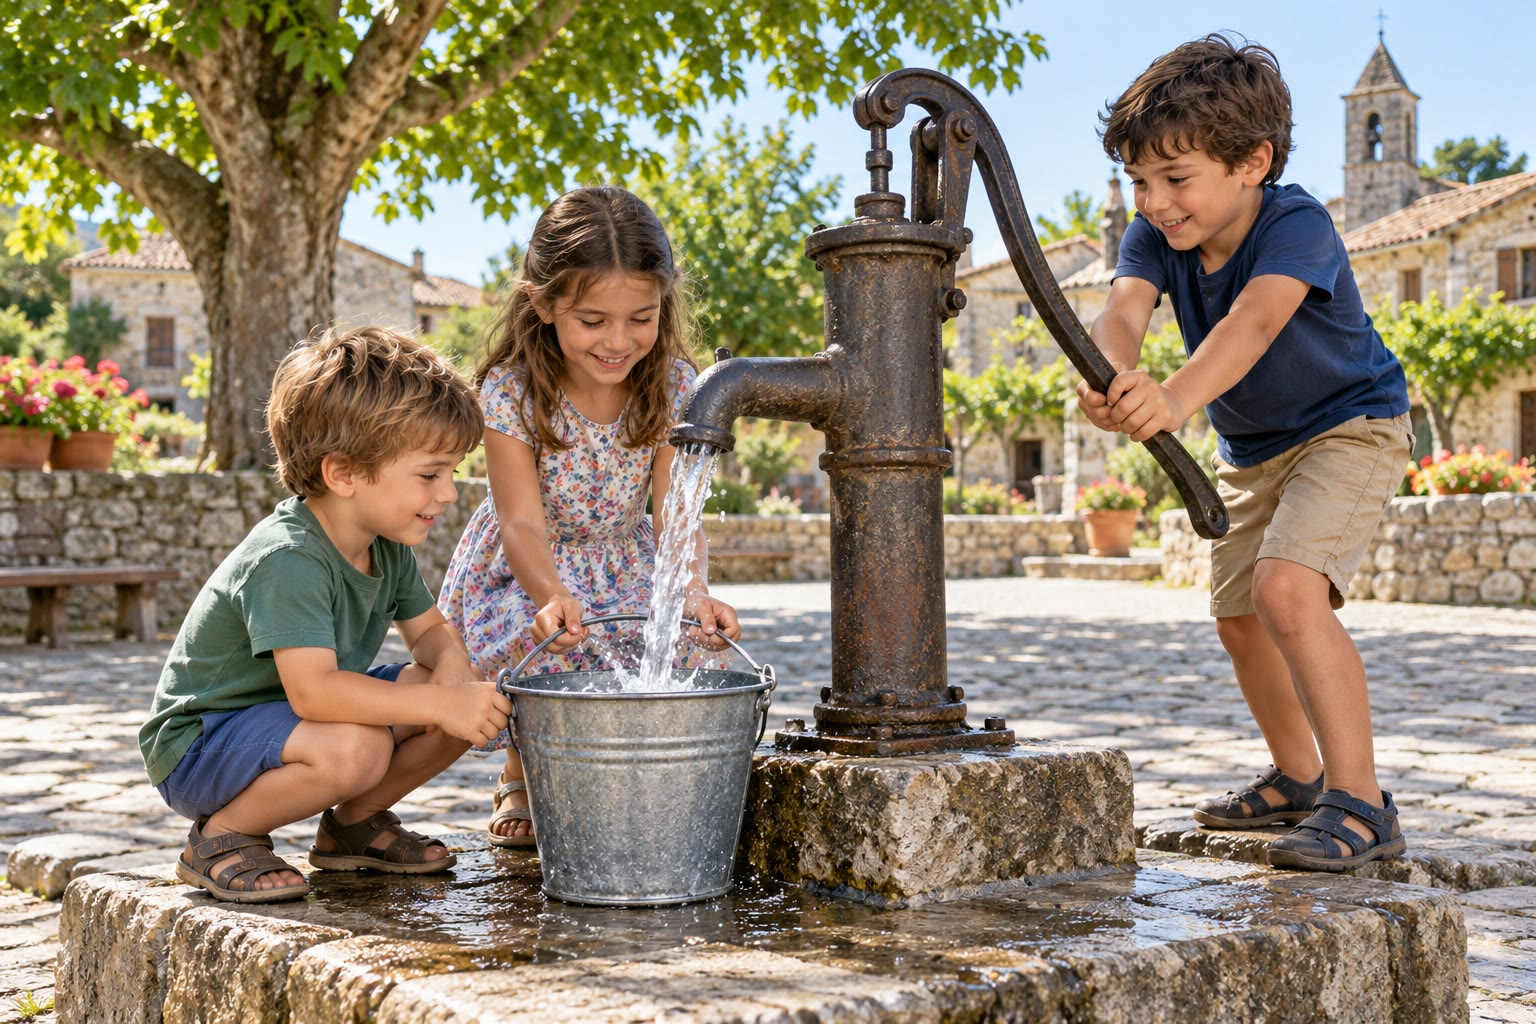
\includegraphics[width=0.6\linewidth]{images/book1/ai/g6-hand-pump.jpg}

{\small 孩子们在乡村\omterm{def:g6:water-underground:spring}{水井}的手压泵旁给水桶装水。（AI
插图。）}
\end{omfigure}

\begin{remark}[水井可能干涸]\label{rem:g6:water-underground:pumping}
从井中抽水会降低其周围的\omterm{def:g6:water-underground:water-table}{地下水位}。若抽水
速度快于雨水补充岩层的速度，\omterm{def:g6:water-underground:water-table}{地下水位}就会不断下降：
井的出水量越来越少，最终可能干涸。两位邻居
从同一岩层抽水，便共享同一水源：一台水泵
就可能使对方的井干涸。
% ledger: wss:aquifer
\end{remark}

\section{含水层}

\begin{definition}[含水层]\label{def:g6:water-underground:aquifer}
\emph{含水层}\index{含水层}是一层多孔且\omterm{def:g6:water-underground:permeability}{透水的}岩层，
其中充满\omterm{def:g6:water-underground:groundwater}{地下水}，并使这些水流向泉和\omterm{def:g6:water-underground:spring}{水井}。
渗入的雨水会补充其水量。
% ledger: wss:aquifer
\end{definition}

瓦尔登\omterm{def:g1:landscapes-around-us:landform}{丘陵}的白垩是一个\omterm{def:g6:water-underground:aquifer}{含水层}：它多孔、透水，
\omterm{def:g1:landscapes-around-us:landform}{丘陵}上的农场正是从中取水。其下的页岩
则不是\omterm{def:g6:water-underground:aquifer}{含水层}，水无法穿过它。
更深处、页岩之下，还有石灰岩和砂岩，它们同样能储水；
要取到这些水，\omterm{def:g6:water-underground:spring}{水井}必须穿透页岩。

\omterm{def:g6:water-underground:groundwater}{地下水}是水循环的一部分。雨水渗入\omterm{def:g6:water-underground:aquifer}{含水层}；
\omterm{def:g6:water-underground:groundwater}{地下水}沿\omterm{def:g6:water-underground:porosity}{孔隙}缓慢流动，从泉涌出或流入\omterm{def:g1:landscapes-around-us:water}{河流}，\omterm{def:g1:landscapes-around-us:water}{河流}再将其带入大海；
在那里，水蒸发后又以雨的形式落下。从\omterm{def:g6:water-underground:aquifer}{含水层}取水，
就像从一个由雨水缓慢注满的水箱中取水：
只有取水不超过雨水所补充的水量，它才能持续供应。

\section{保持地下水清洁}

渗入地下的水在途中会被过滤：树叶、土壤颗粒
和小型生物被土壤与\omterm{def:g3:stones-pebbles-sand:rock}{岩石}拦住。因此，
泉水或井水通常清澈透明。但
水中\emph{溶解的}物质并不会被拦住：它们随水一同
向下迁移，直至\omterm{def:g6:water-underground:water-table}{地下水位}。
% ledger: wss:gw-quality

\omterm{def:g6:water-underground:groundwater}{地下水}可能被人们放在地面上的物质污染：撒在农田和花园里的化肥与
农药、撒在结冰道路上的盐、从油箱中漏出的燃料、露天倾倒的废物，
以及住户管理不善的污水池溢出的水。
这些物质一旦溶解在\omterm{def:g6:water-underground:aquifer}{含水层}中，就很难被去除，
而未经处理的水可能不再适于饮用。
因此，井水在饮用前必须经过检测，化肥、燃料和废物最好远离\omterm{def:g6:water-underground:spring}{水井}和泉水。
% ledger: wss:gw-quality

溶解的物质随\omterm{def:g6:water-underground:groundwater}{地下水}一同迁移。在\omterm{def:g6:water-underground:water-table}{地下水位}以下，
\omterm{def:g6:water-underground:groundwater}{地下水}沿坡向下缓慢渗流：从\omterm{def:g6:water-underground:water-table}{地下水位}较高的
\omterm{def:g1:landscapes-around-us:landform}{丘陵}之下，流向\omterm{def:g6:water-underground:water-table}{地下水位}较低的泉眼与\omterm{def:g1:landscapes-around-us:water}{河流}处。渗入地下的溢出物
因此不会停留在落下的地方，而是下沉至
\omterm{def:g6:water-underground:water-table}{地下水位}，再随\omterm{def:g6:water-underground:groundwater}{地下水}顺坡漂移，流向
坡面上位于其下方的一切。
% ledger: wss:gw-quality, wss:aquifer

\begin{omfigure}
\begin{tikzpicture}[x=1cm, y=1.15cm, font=\scriptsize]
  % ground (the chalk) and the water-filled zone under the water table
  \fill[black!6] (0,0) -- (0,4.090) -- plot[smooth] coordinates {(0.00,4.090) (1.00,4.013) (2.00,3.887) (3.00,3.692) (4.00,3.407) (5.00,3.033) (6.00,2.600) (7.00,2.167) (8.00,1.793) (9.00,1.508) (10.00,1.313) (11.00,1.187) (12.00,1.110)} -- (12,0) -- cycle;
  \fill[blue!14] (0,0) -- (0,3.190) -- plot[smooth] coordinates {(0.00,3.190) (1.00,3.185) (2.00,3.131) (3.00,3.008) (4.00,2.795) (5.00,2.493) (6.00,2.132) (7.00,1.771) (8.00,1.469) (9.00,1.256) (10.00,1.133) (11.00,1.079) (12.00,1.074)} -- (12,0) -- cycle;
  \draw[black!70, line width=0.7pt] plot[smooth] coordinates {(0.00,4.090) (1.00,4.013) (2.00,3.887) (3.00,3.692) (4.00,3.407) (5.00,3.033) (6.00,2.600) (7.00,2.167) (8.00,1.793) (9.00,1.508) (10.00,1.313) (11.00,1.187) (12.00,1.110)};
  \draw[blue!70!black, dashed, line width=0.7pt] plot[smooth] coordinates {(0.00,3.190) (1.00,3.185) (2.00,3.131) (3.00,3.008) (4.00,2.795) (5.00,2.493) (6.00,2.132) (7.00,1.771) (8.00,1.469) (9.00,1.256) (10.00,1.133) (11.00,1.079) (12.00,1.074)};
  % the spill: down to the water table, then downhill with the groundwater
  \fill[brown!70!black, opacity=0.55] (4.85,3.094) -- (5.15,2.971) -- (5.15,2.442) -- (4.85,2.544) -- cycle;
  \fill[brown!70!black, opacity=0.55] (4.85,2.514) -- (5.10,2.429) -- (5.35,2.341) -- (5.60,2.250) -- (5.85,2.158) -- (6.10,2.065) -- (6.35,1.972) -- (6.60,1.881) -- (6.85,1.792) -- (7.10,1.707) -- (7.35,1.626) -- (7.60,1.549) -- (7.85,1.478) -- (8.10,1.413) -- (8.35,1.354) -- (8.60,1.300) -- (8.85,1.252) -- (9.10,1.210) -- (9.30,1.181) -- (9.10,1.182) -- (8.85,1.190) -- (8.60,1.203) -- (8.35,1.221) -- (8.10,1.246) -- (7.85,1.277) -- (7.60,1.313) -- (7.35,1.355) -- (7.10,1.401) -- (6.85,1.486) -- (6.60,1.598) -- (6.35,1.713) -- (6.10,1.828) -- (5.85,1.945) -- (5.60,2.060) -- (5.35,2.174) -- (5.10,2.286) -- (4.85,2.394) -- cycle;
  % the leaking tank
  \draw[fill=black!35] (4.7,3.10) rectangle (5.3,3.42);
  \node[anchor=south, align=center] at (5.0,3.45) {漏油的 \\油箱};
  % groundwater flow
  \begin{scope}[blue!60!black, -{Stealth[length=2mm]}, line width=0.8pt]
    \draw (0.80,2.589) -- (2.40,2.491);
    \draw (3.40,2.334) -- (5.00,1.893);
    \draw (5.90,1.569) -- (7.50,1.009);
    \draw (8.80,0.691) -- (10.60,0.494);
  \end{scope}
  \node[blue!60!black, anchor=north] at (6.7,1.0) {地下水顺坡向下流动};
  % the two wells
  \draw[line width=1.6pt, black!75] (2.0,3.887) -- (2.0,2.70);
  \draw[line width=1.6pt, black!75] (8.5,1.639) -- (8.5,0.95);
  \node[anchor=south, align=center] at (2.0,3.95) {水井 A\\（上坡）：清洁};
  \draw[black!50] (8.5,1.66) -- (8.5,2.30);
  \node[anchor=south, align=center] at (8.5,2.30) {水井 B\\（下坡）：受污染};
  % the stream
  \fill[blue!60] (11.55,1.13) -- (11.95,1.11) -- (11.75,1.02) -- cycle;
  \node[anchor=south] at (11.6,1.20) {溪流};
  \node[blue!70!black, anchor=south west] at (0.1,3.21) {地下水位};
  \node[anchor=west, black!70] at (0.15,0.25) {白垩};
\end{tikzpicture}

{\small 山坡上的溢出物（示意图）。溶解的燃料下沉至
\omterm{def:g6:water-underground:water-table}{地下水位}，再随\omterm{def:g6:water-underground:groundwater}{地下水}顺坡漂移（蓝色箭头）：它
流向坡下的\omterm{def:g6:water-underground:spring}{水井} B，最终进入溪流。\omterm{def:g6:water-underground:spring}{水井} A，
位于油箱上坡，保持清洁。}
\end{omfigure}

\begin{method}[水井是否有风险？]\label{met:g6:water-underground:risk}
\begin{enumerate}
  \item 找出\omterm{def:g6:water-underground:water-table}{地下水位}高的地方与低的地方：高的地方位于
        \omterm{def:g1:landscapes-around-us:landform}{丘陵}之下，低的地方位于泉眼与\omterm{def:g1:landscapes-around-us:water}{河流}附近。
  \item \omterm{def:g6:water-underground:groundwater}{地下水}由高处流向低处：用
        箭头标出它的流动方向。
  \item 位于污染源下坡、且处于该箭头
        路径上的\omterm{def:g6:water-underground:spring}{水井}或泉眼有风险；位于其上坡的\omterm{def:g6:water-underground:spring}{水井}则没有。
\end{enumerate}
\end{method}

\begin{example}[农场的新油箱]\label{ex:g6:water-underground:tank}
一位农民住在白垩质山坡上，饮用自家\omterm{def:g6:water-underground:spring}{水井}中的水，该井位于
半山坡处。她想在两块田地中选一块设置新油箱：一块
位于\omterm{def:g6:water-underground:spring}{水井}上坡，另一块位于\omterm{def:g6:water-underground:spring}{水井}下坡、靠近溪流处。\omterm{def:g6:water-underground:groundwater}{地下水}
顺坡向下流动。上坡田地的泄漏物会向下漂移，流向
\omterm{def:g6:water-underground:spring}{水井}；下坡田地的泄漏物则会远离\omterm{def:g6:water-underground:spring}{水井}，流向
溪流。对\omterm{def:g6:water-underground:spring}{水井}而言，\omterm{def:g6:water-underground:spring}{水井}下坡的田地是更好的选择
——而把油箱放在可承接任何泄漏物的托盘上则更为稳妥，
因为溪流同样重要。
\end{example}

\begin{inthefield}[辨认泉眼]
与成人一同散步时，沿山坡坡脚观察。泉眼常表现为
一片潮湿的地面、干燥田地中一线较绿的草或芦苇、
一条不知从何处冒出的小溪，或是为承接泉水而砌的石盆
或水槽。在详细的步行\omterm{def:g2:drawing-to-map:map}{地图}上，泉眼用一个小符号标出。
在小路上观察即可，切勿饮用
未经检测的泉水。
\end{inthefield}

\section{练习}

\begin{exercise}[$\star$]\label{exo:g6:water-underground:1}
将下列材料分为“\omterm{def:g6:water-underground:permeability}{透水的}”和“\omterm{def:g6:water-underground:permeability}{不透水的}”两类：沙、
黏土、\omterm{def:g3:stones-pebbles-sand:pebble}{砾石}、无裂隙的花岗岩、页岩、白垩。
\end{exercise}

\begin{exercise}[$\star$]\label{exo:g6:water-underground:2}
将每个词与其含义配对：泉、\omterm{def:g6:water-underground:spring}{水井}、\omterm{def:g6:water-underground:water-table}{地下水位}、\omterm{def:g6:water-underground:aquifer}{含水层}。
(a) 所有\omterm{def:g6:water-underground:porosity}{孔隙}都充满水的区域的顶部。(b) 一层
多孔且透水、能储存\omterm{def:g6:water-underground:groundwater}{地下水}的岩层。(c) \omterm{def:g6:water-underground:groundwater}{地下水}
自行流出的地方。(d) 一个向下延伸至\omterm{def:g6:water-underground:water-table}{地下水位}以下的
孔洞。
\end{exercise}

\begin{exercise}[$\star$]\label{exo:g6:water-underground:3}
(a) 说出雨水落到陆地上后可能经过的三条路径。
(b) 暴雨过后，径流更多地出现在停车场还是草地上？
为什么？
\end{exercise}

\begin{exercise}[$\star$]\label{exo:g6:water-underground:4}
判断下列说法正误，并改正错误的句子。(a) 多孔\omterm{def:g3:stones-pebbles-sand:rock}{岩石}
总是\omterm{def:g6:water-underground:permeability}{透水的}。(b) \omterm{def:g6:water-underground:water-table}{地下水位}以下，\omterm{def:g6:water-underground:porosity}{孔隙}中充满水。
(c) \omterm{def:g6:water-underground:water-table}{地下水位}是平的，像湖面一样。(d) 地下的\omterm{def:g2:water-on-earth:salt-fresh}{淡水}
比全部\omterm{def:g1:landscapes-around-us:water}{湖泊}中的\omterm{def:g2:water-on-earth:salt-fresh}{淡水}还多。
\end{exercise}

\begin{exercise}[$\star\star$]\label{exo:g6:water-underground:5}
一只桶里装有 10~升干沙。沙的\omterm{def:g6:water-underground:porosity}{孔隙度}为 25~\%。
往桶里最多能倒入多少水才会溢出？若在桶底开一个小孔，
则有多少水会从孔中流出（22~\%）？
\end{exercise}

\begin{exercise}[$\star\star$]\label{exo:g6:water-underground:6}
一块石灰岩尺寸为 2~m × 1~m × 1~m。(a) 其体积是多少，
分别以立方米和升表示？(b) 其\omterm{def:g6:water-underground:porosity}{孔隙度}为 20~\%，装满时\omterm{def:g6:water-underground:porosity}{孔隙}中能容纳多少升
水？(c) 这些水中有 18~\% 的体积会流出。
流出多少升？还有多少升滞留在\omterm{def:g3:stones-pebbles-sand:rock}{岩石}中？
\end{exercise}

\begin{exercise}[$\star\star$]\label{exo:g6:water-underground:7}
利用穿过瓦尔登\omterm{def:g1:landscapes-around-us:landform}{丘陵}的剖面。(a) 泉和\omterm{def:g1:landscapes-around-us:water}{河流}分别位于
什么高程？(b) 泉位于\omterm{def:g1:landscapes-around-us:water}{河流}上方还是下方？泉水
流向何处？(c) 为什么白垩
山坡中部没有泉？
\end{exercise}

\begin{exercise}[$\star\star$]\label{exo:g6:water-underground:8}
井~A 处地面高程为 401~m，雨季后\omterm{def:g6:water-underground:water-table}{地下水位}高程为 336~m，
旱季后为 314~m。(a) 各季节中\omterm{def:g6:water-underground:water-table}{地下水位}
在地面以下多深？(b) \omterm{def:g6:water-underground:water-table}{地下水位}在两季之间
下降了多少米？
\end{exercise}

\begin{exercise}[$\star\star$]\label{exo:g6:water-underground:9}
一位农夫想在山顶，即剖面的
右端打一口新井。这口井必须比井~A 更深还是更浅？请结合
\omterm{def:g6:water-underground:water-table}{地下水位}加以说明。
\end{exercise}

\begin{exercise}[$\star\star$]\label{exo:g6:water-underground:10}
一立方米黏土可容纳 500~升水，却只能出水 20~升。
试解释为什么挖在黏土中的井几乎不出水，
尽管黏土中充满了水。
\end{exercise}

\begin{exercise}[$\star\star\star$]\label{exo:g6:water-underground:11}
在地球全部\omterm{def:g2:water-on-earth:salt-fresh}{淡水}中，30.1~\% 为\omterm{def:g6:water-underground:groundwater}{地下水}，0.26~\% 位于
\omterm{def:g1:landscapes-around-us:water}{湖泊}中。(a) 地下\omterm{def:g2:water-on-earth:salt-fresh}{淡水}的量是\omterm{def:g1:landscapes-around-us:water}{湖泊}中\omterm{def:g2:water-on-earth:salt-fresh}{淡水}量的
多少倍？(b) 全部\omterm{def:g2:water-on-earth:salt-fresh}{淡水}中约 69~\% 为冰雪，
其余部分（\omterm{def:g6:water-underground:groundwater}{地下水}、\omterm{def:g1:landscapes-around-us:water}{湖泊}、\omterm{def:g1:landscapes-around-us:water}{河流}、空气、
土壤\ldots）占多大份额？(c) 为什么\omterm{def:g6:water-underground:groundwater}{地下水}对饮用水如此重要？
\end{exercise}

\begin{exercise}[$\star\star\star$]\label{exo:g6:water-underground:12}
两座农场并排位于同一片白垩地上。一个夏天，第一座农场安装了
一台大功率水泵并注满了一个大池塘；几周后，第二座农场的
井干涸了，尽管没有人动过它。试解释发生了什么，
以及两位农场主可以采取哪些措施。
\end{exercise}

\section{问题：瓦尔登丘陵的农场水井}

\begin{problem}[{周末问题——瓦尔登丘陵农场下方的岩石、
其白垩中储存的水，以及在
无雨情况下能维持多少天}]
\label{pb:g6:water-underground:1}
% ledger: heath:porosity, wss:aquifer
瓦尔登\omterm{def:g1:landscapes-around-us:landform}{丘陵}的一座农场位于白垩层上，紧邻
剖面中的井~A。农场主想知道，遇到长期\omterm{def:g5:natural-hazards:drought}{干旱}时，
这口井能让农场维持多久，若白垩层完全得不到降雨补给。

\medskip
\noindent\textbf{第一部分——农场下的\omterm{def:g3:stones-pebbles-sand:rock}{岩石}。}
\begin{enumerate}
  \item 说出农场所在的\omterm{def:g3:stones-pebbles-sand:rock}{岩石}及其下方的\omterm{def:g3:stones-pebbles-sand:rock}{岩石}。其中哪一种
        是\omterm{def:g6:water-underground:permeability}{透水的}？
  \item 解释为什么在农场下方的坡脚处有泉水涌出。
  \item 利用剖面：农场处地面高程为 401~m，雨季后
        \omterm{def:g6:water-underground:water-table}{地下水位}高程为 336~m。\omterm{def:g6:water-underground:water-table}{地下水位}在地面以下多深？
  \item 旱季后，\omterm{def:g6:water-underground:water-table}{地下水位}高程为 314~m。井~A
        深 100~m，它是否仍能取到水？水面高出井底多少米？
\end{enumerate}

\medskip
\noindent\textbf{第二部分——白垩中的水。}
农场主可以在\omterm{def:g6:water-underground:water-table}{地下水位}以下，抽取井周围一个长 100~m、
宽 50~m、厚 2~m 的白垩块体中的水。白垩是一种石灰岩，
计算时取\omterm{def:g6:water-underground:porosity}{孔隙度}为 20~\%，可流出水所占的比例为 18~\%。
\begin{enumerate}[resume]
  \item 该块体的体积是多少立方米？
  \item 其\omterm{def:g6:water-underground:porosity}{孔隙}中充满的水有多少立方米？
  \item 有多少立方米的水流入井中？又有多少
        立方米滞留在白垩中？
  \item 将流出的水量换算为升。
\end{enumerate}

\medskip
\noindent\textbf{第三部分——能维持多久。}
\begin{enumerate}[resume]
  \item 农场（住房、牲畜和菜园）每天用水
        18~立方米。这相当于多少升？
  \item 农场一周用水多少？
  \item 为什么白垩中的储水在正常
        年份里不会用完？
  \item 若完全没有降雨，流出该块体的水能
        供农场使用多少天？
\end{enumerate}
\end{problem}
